\documentclass[tikz,border=10pt]{standalone}
\usepackage{amsmath}
\usepackage{amssymb}
\definecolor{mantis}{RGB}{0, 105, 62}
\begin{document}
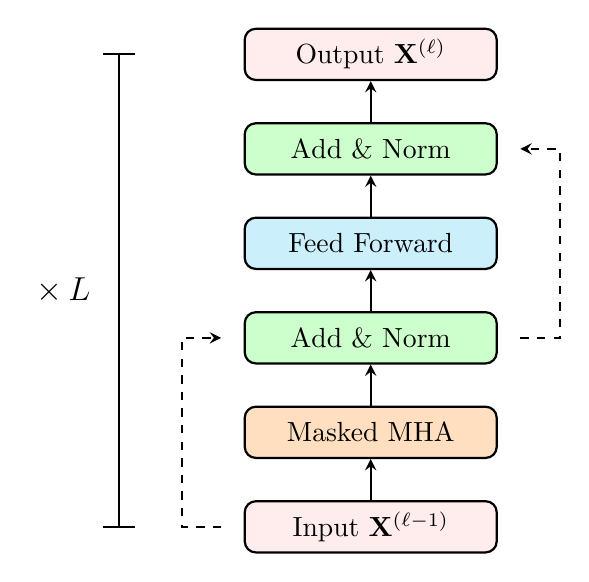
\begin{tikzpicture}[>=stealth,
    block/.style={draw, rounded corners, minimum width=3.2cm, minimum height=0.65cm, thick}]
    \node[block, fill=pink!30] (input) at (0,0) {Input $\mathbf{X}^{(\ell-1)}$};
    \node[block, fill=orange!25] (mha) at (0,1.2) {Masked MHA};
    \node[block, fill=green!20] (an1) at (0,2.4) {Add \& Norm};
    \node[block, fill=cyan!20] (ffn) at (0,3.6) {Feed Forward};
    \node[block, fill=green!20] (an2) at (0,4.8) {Add \& Norm};
    \node[block, fill=pink!30] (output) at (0,6.0) {Output $\mathbf{X}^{(\ell)}$};
    \draw[->, thick] (input) -- (mha);
    \draw[->, thick] (mha) -- (an1);
    \draw[->, thick] (an1) -- (ffn);
    \draw[->, thick] (ffn) -- (an2);
    \draw[->, thick] (an2) -- (output);
    \draw[->, thick, dashed] (-1.9,0) -- (-2.4,0) -- (-2.4,2.4) -- (-1.9,2.4);
    \draw[->, thick, dashed] (1.9,2.4) -- (2.4,2.4) -- (2.4,4.8) -- (1.9,4.8);
    \draw[thick] (-3.2,0) -- (-3.2,6.0);
    \draw[thick] (-3.4,0) -- (-3.0,0);
    \draw[thick] (-3.4,6.0) -- (-3.0,6.0);
    \node[font=\large] at (-3.9,3.0) {$\times\, L$};
\end{tikzpicture}
\end{document}
